% !TEX root = ../main.tex

\chapter{编译链概览} \label{ch:overview}

我们构建了一个从函数式语言PCF到LLVM IR的部分经过验证的编译器,并在Coq定理证明工具中
完成了编译算法和形式化验证的实现~\cite{chlipala2022certified}。
在本章中,我们主要是从高层次的角度介绍了这个编译器原型,省略了转换算法设计和证明定理的详细信息。
CPS转换及CPS到SSA转换的正确性通过源程序和目标程序之间的模拟进行形式化验证,
遵循第\ref{sec:compcertbackend}节中所介绍的CompCert后端的验证框架。
我们使用$\approx $表示语义保存性质。PCF、CPS和SSA的程序分别表示为$t_{pcf}$、$t_{cps}$和$t_{ssa}$。
通过对$t_{pcf}\approx t_{cps}$和$t_{cps}\approx t_{ssa}$的形式化证明,可以组合推导出$t_{pcf}\approx t_{ssa}$。
然后我们就得到了一个从PCF到SSA的经验证的编译过程。我们应用该经验证的编译过程,构建出一个编译器原型。
该编译器读取PCF程序,并经过图\ref{overview}中所示的几个编译步骤生成LLVM IR程序。

\begin{figure}[htbp]
    \centering
    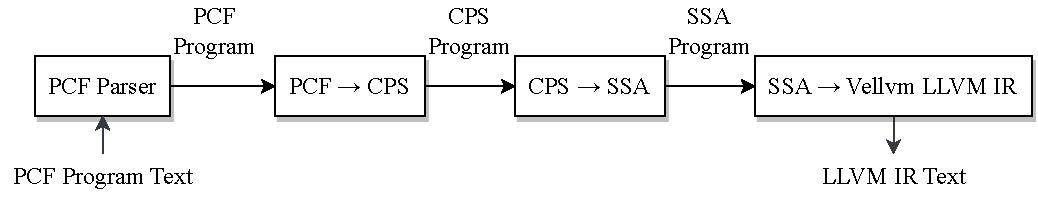
\includegraphics[width=0.8\linewidth]{figures/overview.pdf}
    \caption{PCF到LLVM编译链概览}\label{overview}
\end{figure}

\section{PCF语法分析器}

该PCF语法分析器(Parser)将文本形式的PCF程序提取为Coq中的结构化PCF代码项。
为了分析文本信息并提取PCF程序,获取源程序的语法结构至关重要。对于文本形式的PCF程序,
我们首先用词法分析器(Lexical Parser)将其解析为令牌(Token)流。
随后,使用语法分析器(Syntax Parser)分析该令牌流,生成Coq中的直接风格PCF程序项。

\section{CPS转换}

如第\ref{sec:background}节中所言,函数式编程语言的编译器通常会将直接风格的程序转换为CPS形式,以获得显式的控制流。
将直接形式的PCF程序转换为CPS形式的算法主要由当前代码项和当前项被规约为某个值后要处理的下一个项决定。
关于该CPS转换算法及其正确性验证的详细信息将在第\ref{sec:cpstrans}节和第\ref{sec:cpsforward}节中进行讨论。

\section{从CPS到SSA}

目标SSA语言是LLVM IR的简化版本,保留了其最基本的结构和程序语句。
通过该编译过程,输入的CPS程序项将被转换为一个包含主函数的SSA程序。
在第\ref{sec:cpsssatrans}节中将详细介绍该转换算法的设计和细节。
第\ref{sec:cpsssaforward}节中将进行CPS到SSA转换算法的形式化验证,并通过运行一个示例程序展示前向模拟的每一个关键步骤。

\section{从SSA到LLVM IR}

SSA程序被转换为Vellvm中的抽象语法树,然后转换为LLVM IR程序文本。
在该编译链中,我们使用了经过验证的LLVM基础设施Vellvm~\cite{zakowski2021modular})。
利用其在Coq实现的LLVM IR的抽象语法树,我们可以进一步输出最终的LLVM IR程序。
